\title{Adders}
\begin{document}
\section{Simple Adders}
\subsection{Half Adders}

\begin{frame}{Half adders}
  \begin{definition}
    A \alert{half adder} adds two one bit operands to produce a one bit half sum (HS) and a one bit carry out (CO).
  \end{definition}
  The logic equations for a half adder, with operands X and Y look like this:
  $$HS = X \oplus Y$$
  $$CO = X \cdot Y$$
  Notice that we have no carry in, so we can only use this idea to add two bits.
\end{frame}

Show the truth tables for XOR and AND to see how we get these results.

\subsection{Full Adders}

\begin{frame}{Full adder}
  \begin{definition}
    A \alert{full adder} adds three one bit operands (X, Y, and CIN) to produce a sum (S) and a carry out (CO).
  \end{definition}
  These are the logic equations for a full adder:
  $$S = X \oplus Y \oplus CIN$$
  $$COUT = X \cdot Y + X \cdot CIN + Y \cdot CIN$$
\end{frame}

\begin{frame}{Representations of a full adder}
  \begin{columns}
    \begin{column}{6cm}
      \begin{center}
        Logic diagram:\\
        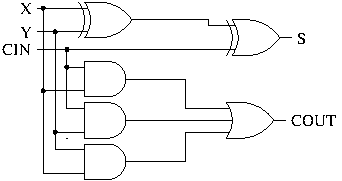
\includegraphics{FullAdderLogic}
      \end{center}
    \end{column}
    \begin{column}{6cm}
      \begin{center}
        Schematic diagram:\\
        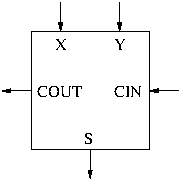
\includegraphics{FullAdderSchematic}
      \end{center}
    \end{column}
  \end{columns}
\end{frame}

\section{Ripple Adders}

\begin{frame}{Ripple adders}
  To perform addition on operands of more than one bit, we can cascade full adders.
  \begin{center}
    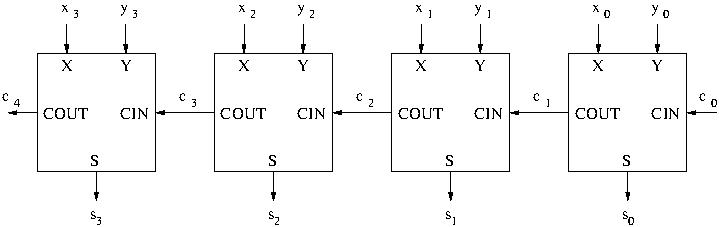
\includegraphics[scale=0.8]{RippleAdderSchematic}
  \end{center}
  What is a possible problem with this design?
\end{frame}

\section{Subtractors}

\begin{frame}{Subtractors}
  We can perform the subtraction $D = X - Y$ with a borrow in of BIN and a borrow out of BOUT using the following logic equations.\\
  $$D = X \oplus Y \oplus BIN$$
  $$BOUT = X' \cdot Y + X' \cdot BIN + Y \cdot BIN$$
\end{frame}

\begin{frame}{Implementing a subtractor with an adder}
  \begin{block}{The Joy of Two's Complement}
    Recall that we can perform $X - Y$ by doing $X + \overline{Y} + 1$ if X and Y are two's complement binary numbers.
  \end{block}
  \begin{center}
    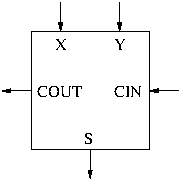
\includegraphics{FullAdderSchematic}
  \end{center}
\end{frame}

\begin{frame}{The real subtractor}
  \begin{center}
    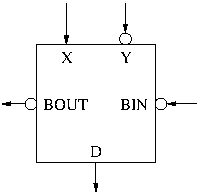
\includegraphics{SubtractorSchematic}
  \end{center}
\end{frame}

\section{Carry-Lookahead Adders}

\begin{frame}{Back to the Future}
  \begin{block}{Hey McFly...}
    Any given sum will either generate or propagate a carry out.\\
    $g_i = x_i \cdot y_i$\\
    $p_i = x_i + y_i$
  \end{block}
  \begin{block}{Great Scott!}
    Then we can look into the future and determine the carry out of any stage.
    $$c_{i+1} = g_i + p_i \cdot c_i$$
  \end{block}
  \begin{block}{1.21 Gigawatts}
    So then for each stage, we can \alert{immediately} compute the carry out based only on the original operands.
  \end{block}
\end{frame}

Show the carry-out expansion.

\section{MSI Components}
\subsection{The 74x83 Adder}

\begin{frame}{The 74x283 adder}
  \begin{center}
    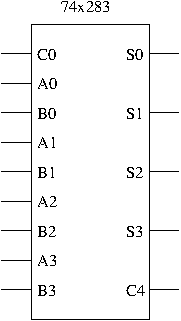
\includegraphics{74x283Schematic}
  \end{center}
\end{frame}

\subsection{The74x181 ALU}

\begin{frame}{The 74x181 ALU}
  \begin{center}
    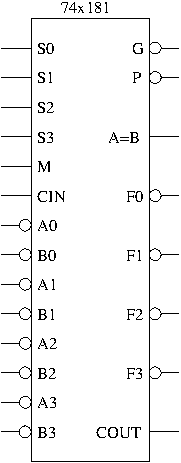
\includegraphics[scale=0.8]{74x181Schematic}
  \end{center}
\end{frame}

\end{document}
